\documentclass{article}
\usepackage{tikz}
\usepackage{pgfplots}
\usepackage{xcolor}
\usepackage{svg}
\usepackage{amsmath}
\usepackage{array}
\usepackage[skins]{tcolorbox}
\usepackage[version=4]{mhchem}
\usepackage[a4paper, total={6in, 9in}]{geometry}
\usepackage{fourier}
\usepackage{xymtex}
\usepackage{textcomp}
\usepackage{eurosym}
\usepackage{caption}
\usepackage{longtable}
\usepackage{float}
\usepackage{attachfile}
\usepackage{multirow}
\usepackage{float}
\usepackage{amsfonts} 
\pgfplotsset{compat=1.18}

\captionsetup[table]{name=\textit{Tabella}}
\pagenumbering{gobble}
%\setcounter{secnumdepth}{2}

\title{Relazione di laboratorio - Esperienza di Poisson}
\author{Federico Cesari}
\date{Marzo 2024}




\begin{document}
\begin{titlepage}
	\begin{center}
		\vspace*{1cm}
		
		\textbf{\LARGE Relazione di laboratorio - Pendolo semplice}
		
		\vspace{0.3cm}
		\large \textit{Misura del periodo di un pendolo semplice} \\
		
		\vspace{0.5cm}
		\Large Federico Cesari \\
		
		\small 1096759 
		\vspace{0.2cm}
		
		\small Gruppo 5
		
		
		\vspace{3cm}
		\begin{center}
			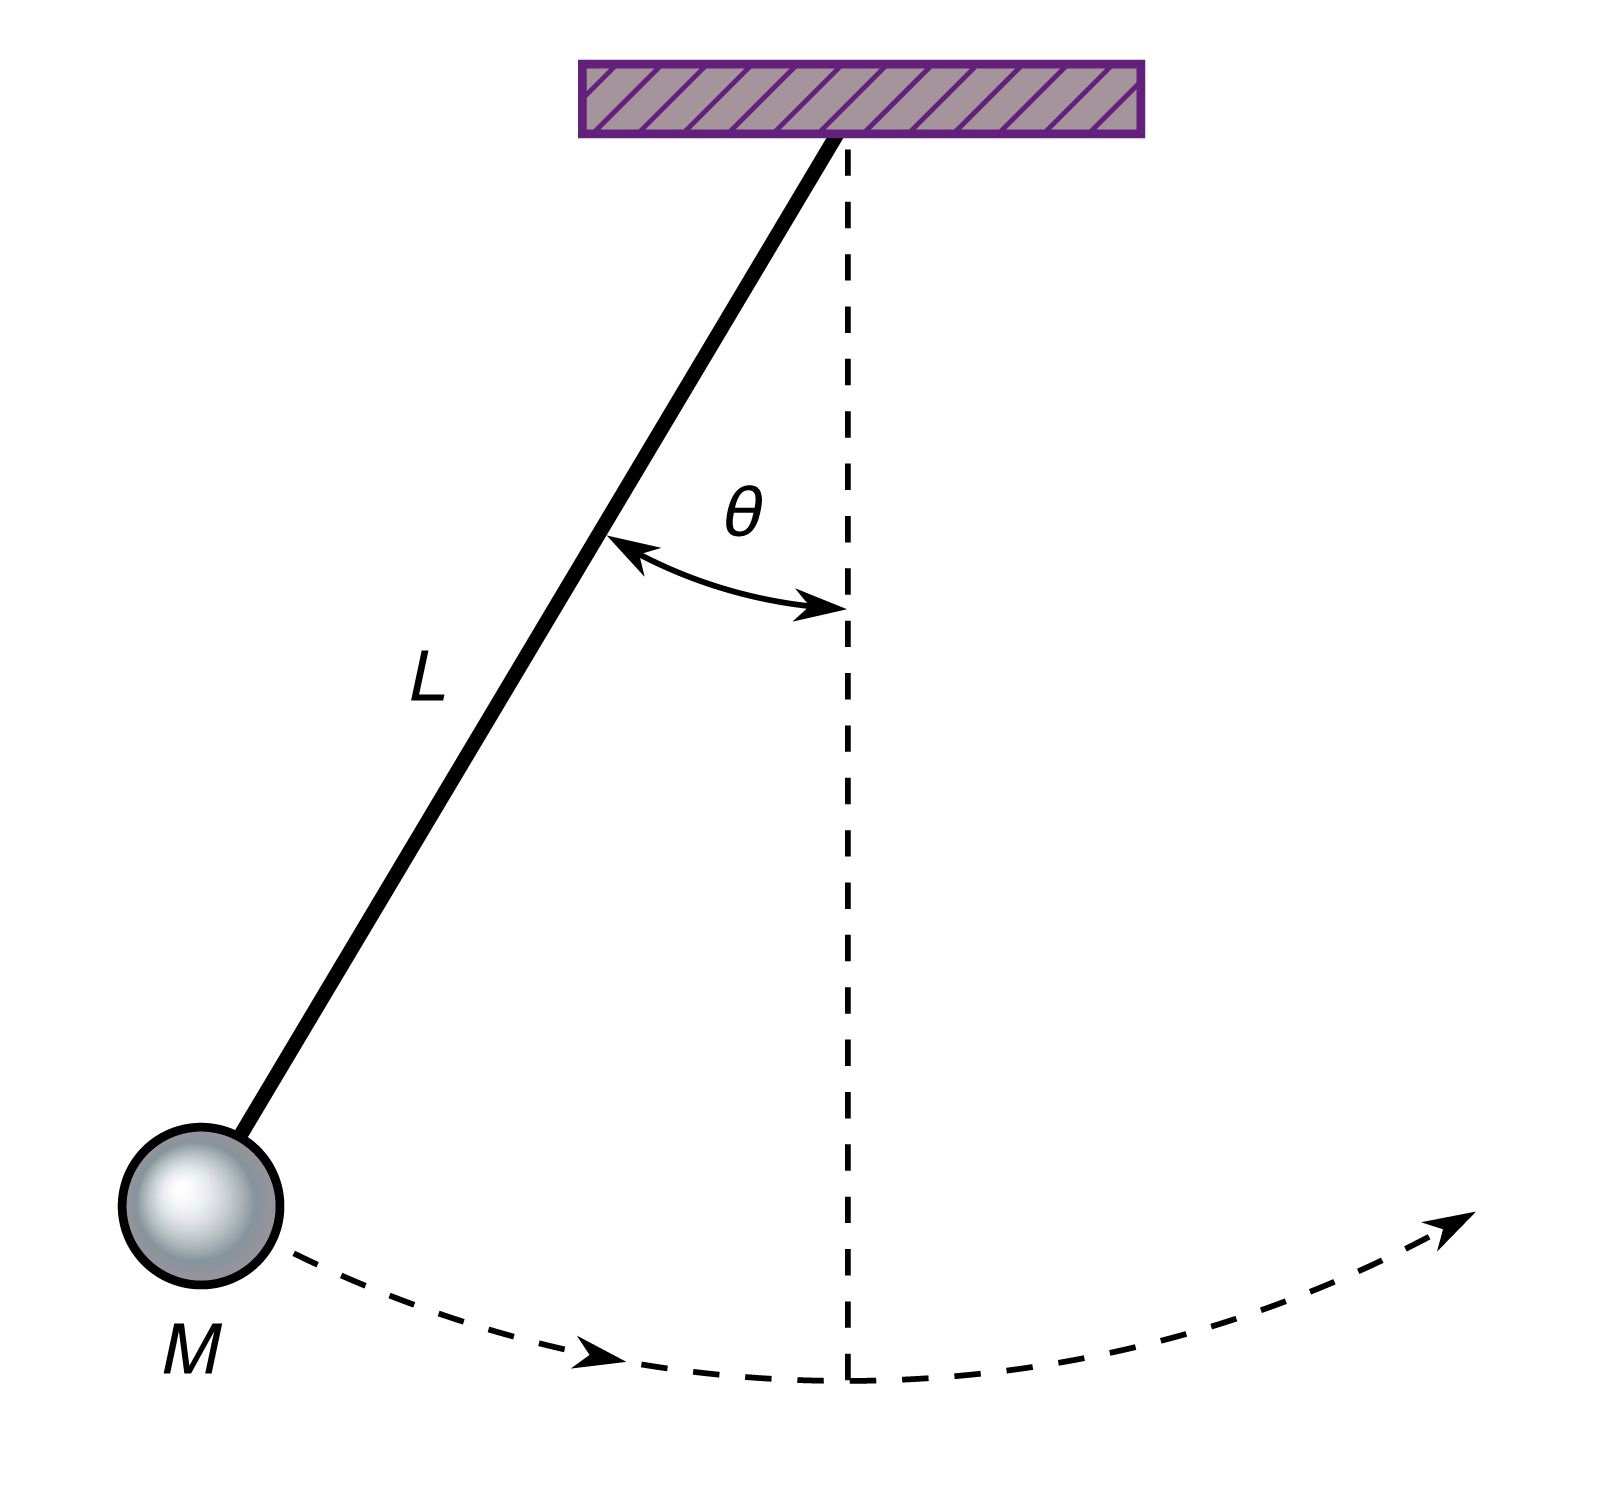
\includegraphics[scale=0.1]{IMG_0200.jpeg}	
		\end{center}
		
		
		
		\vfill
		
		
		
		corso A\\
		Università degli studi di Torino, Torino\\
		4 aprile 2024\\
		
		
	\end{center}
\end{titlepage}

%Scopo : misurare il rate 
%rilevatore di radiazioni: contatore geiger
%rotaia con uranile a 3cm

%Calcolare il rate del fondo: rapporto tra media e deviazione standard e tempo porta.

%\section{Test $\chi^2$}
%!incertezza per somma e differenza è la radice quadrata della somma dei quadrati delle incertenza. 
%\begin{enumerate}
%	\item 	rate fondo (tempo porta = 1s): $RF(1sec) = 0.305 \pm 0.014 s^{-1}$. (\textit{nonost			   ante preferisca una sola cifra significativa per l'errore lascio 0.014, sottostimer			      ei di troppo se arrotondassi}.)
%	\item rate fondo + sorgente (tempo porta = 1s): $RFS(<1sec) = 3.145 \pm 0.045 s^{-1}$
%\end{enumerate}
%\[
%RS(1sec) = RFS(1sec) - RF(1sec) 
%\]

%con errore
%\[
%\delta_{RS(1sec)} =\sqrt{\delta_{RFS(1sec)}^2 + \delta_{RF(1sec)}^2}
%\]
\textcolor{white}{.}
\vfill
\section{Scopo dell'esperienza}
L'esperienza di laboratorio ha come scopo la misurazione del rate di una sorgente radioattiva, ovvero il numero di eventi registrati in tempi porta di $1$ e $3$ secondi dal contatore geiger quando la sorgente è posta a \(3\)cm da questo. 

L'apparato sperimentale utilizzato consiste di: 

\begin{enumerate}
	\item Contatore geiger: registra grazie a degli impulsi elettrici gli eventi radioattivi;
	\item Pietra uranile: posta su un sostegno è la sorgente radioattiva utilizzata;
	\item Rotaia su cui sono posti il contatore e il sostegno così da permettere la regolazione della distanza della sorgente dal contatore;
	\item Computer: per memorizzare e analizzare i conteggi del contatore geiger.
\end{enumerate}

\paragraph{Aspettative}
La probabilità di misurare un conteggio in una serie di intervalli di tempo (nel nostro caso i due tempi porta) rappresenta la probabilità di rilevare $p$ successi in $n$ prove. Poiché posso o avere o non avere un conteggio la distribuzione che descrive il fenomeno è quella binomiale. 

Inoltre la probabilità di successo risulta essere molto bassa e affiancata ad un numero di prove piuttosto elevato (1500). Proprio a causa di questi valori la distribuzione binomiale che descrive i miei dati dovrebbe avvicinarsi sempre di più all'andamento di una distribuzione di Poisson e, all'aumentare del valor medio, addirittura a quello di una distribuzione Normale. Procederò alla verifica dell'addattamento delle due distribuzioni limite tramite un test del $\chi^2$.

\section{Acquisizione dati}
Prima di effettuare le misurazioni del rate della sorgente radioattiva misuro il rate dovuto solamente alla radioattività naturale di fondo. La radiazione di fondo è causata dalla presenza di gas radioattivi come Radon e Torio in atmosfera, dalla presenza di elementi radioattivi nel terreno e in acqua, oppure da radiazioni cosmiche che portano  particelle ad alta energia cariche positivamente che entrano in atmosfera provocando l'emissione di fotoni, elettroni e neutroni. 

Nel momento in cui dovrò misurare il rate dell'uranile dovrò tenere in considerazione la presenza dei conteggi dovuti al fondo che si andranno a "sommare". \\

\noindent
Il rate per ciascun tempo porta è calcolato come
\[
	\text{Rate} = \frac{\bar{x}}{\tau} \pm \frac{\sigma_{\bar{x}}}{\tau}
\]
dove $\bar{x}$ è il valor medio, $\sigma_{\bar{x}}$ è la deviazione standard della media e $\tau$ è il tempo porta.

% FONDO
\section{Distribuzione sperimentale del fondo}
Senza avvicinare la sorgente radioattiva al contatore geiger prendo 1500 misurazioni, prima con tempo porta di 1s e poi di 3s, del rate dei conteggi radioattivi dovuti unicamente alla radiazione di fondo ottenendo i valori riportati in \textit{Tabella 1} e \textit{Tabella 2}. 


%ISTOGRAMMI 1
\vspace{0.5cm}
\hspace{-0.7cm}
\begin{minipage}[c]{0.45\textwidth}
\begin{center}
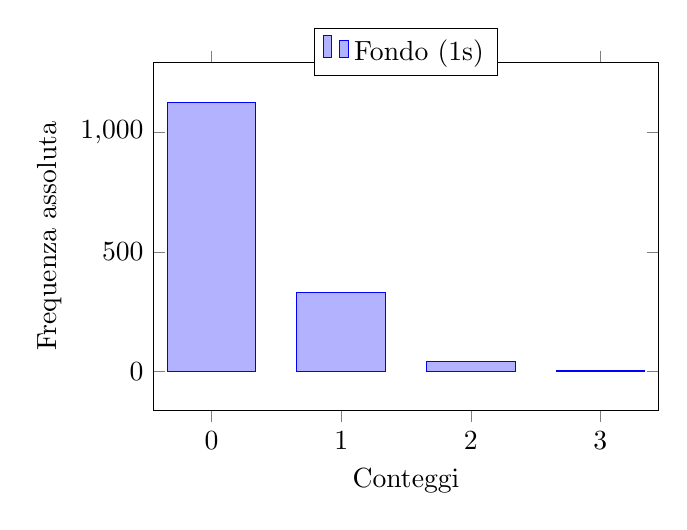
\begin{tikzpicture}
\begin{axis}[
	width=8cm, 
	height=6cm,
	ylabel=Frequenza assoluta,
	xlabel=Conteggi,
	enlargelimits=0.15,
	legend style={at={(0.5,1.1)},anchor=north,legend columns=-1},
	ybar=0pt,% configures `bar shift'
	bar width=32pt,
	xtick={0,1,2,3},
	xticklabels={0,1,2,3},
	xticklabel style={rotate=0,align=center}]
	\addplot
	coordinates {
		(0,1125)
		(1,330)
		(2,41)
(3,4)};
	\legend{Fondo (1s)}
\end{axis}
\end{tikzpicture}
\end{center}
\end{minipage}
\hfill
\begin{minipage}[c]{0.45\textwidth}
\begin{center}
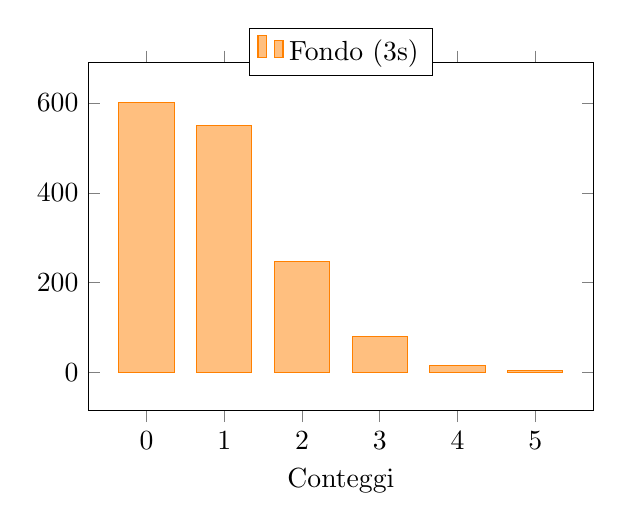
\begin{tikzpicture}
\begin{axis}[
	width=8cm, 
	height=6cm,
	xlabel=Conteggi,
	enlargelimits=0.15,
	legend style={at={(0.5,1.1)},	anchor=north,legend columns=-1},
	ybar=0pt,% configures `bar shift'
	bar width=20pt,
	xtick={0,1,2,3,4,5},
	xticklabels={0,1,2,3,4,5},
	xticklabel style={rotate=0,align=center}]
	\addplot+[opacity=0.5,fill=orange,draw opacity=1,draw=orange] 
	coordinates {
		(0,601)
		(1,551)
		(2,247)
		(3,81)
		(4,15)
		(5,5)};
	\legend{Fondo (3s)}
\end{axis}
\end{tikzpicture}
\end{center}
\end{minipage}


%TABELLE 1
\begin{minipage}[c]{0.45\textwidth}
\vspace{1cm}
\begin{center}
\hspace{0.5cm}
\begin{tabular}{llr}
	Media                       & $\bar{x}$             & $0.283$       \\		
	Varianza                    & $\sigma_{x}^2$          & $0.274$     \\
	Dev. std                    & $\sigma_{x}$              & $0.523$   \\
	Dev. std (della media)      & $\sigma_{\bar{x}}$    & $0.014$       \\
\end{tabular}
\captionof{table}{\textit{Fondo (1s)}}
\end{center}

\[ 
	\text{\textbf{Rate del fondo (1s)}} \mathbf{ = \left(0.283 \pm 0.014\right)}\text{ \textbf{count/s}}
\]
\end{minipage}
\hfill
\begin{minipage}[c]{0.45\textwidth}
\vspace{1cm}
\begin{center}
\begin{tabular}{llr}
	Media                       & $\bar{x}$             & $0.915$       \\		
	Varianza                    & $\sigma_{x}^2$          & $0.918$     \\
	Dev. std                    & $\sigma_{x}$              & $0.958$   \\
	Dev. std (della media)      & $\sigma_{\bar{x}}$    & $0.025$       \\
\end{tabular}
\captionof{table}{\textit{Fondo (3s)}}
\end{center}

\[ 
	\text{\textbf{Rate del fondo (3s)}}  \mathbf{ = \left(0.305 \pm 0.01 \right)} \text{ \textbf{count/s}}
\]
\end{minipage}
\footnote{Per il rate del fondo con tempo porta di 1s non approssimo l'incertezza a una sola cifra significativa perché porterei la sottostima dell'errore al 40\% e andrei a considerare un valore troppo poco accurato.}



% FONDO + SORGENTE    3cm
\newpage
\section{Distribuzione sperimentale di fondo + sorgente a 3cm}
Posizionata la pietra uranile su un sostegno a 3cm dal contatore misuro 1500 eventi prima con tempo porta di 1s e poi con tempo porta di 3s. 

\vspace{0.6cm}
\hspace{-0.5cm}
\begin{minipage}[c]{0.5\textwidth}
\begin{center}
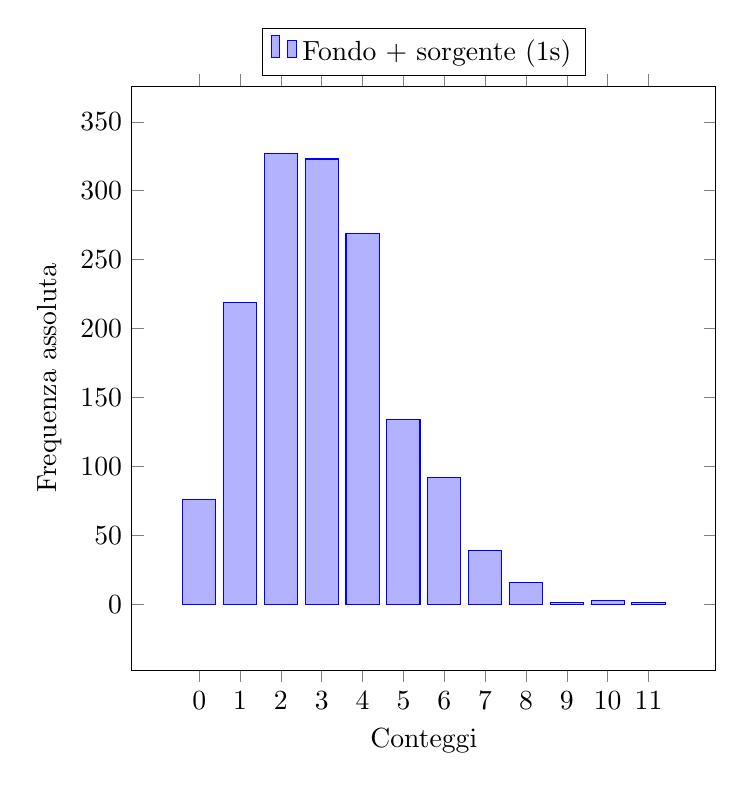
\begin{tikzpicture}
\begin{axis}[
	width=9cm, 
	height=9cm,
	ylabel=Frequenza assoluta,
	xlabel=Conteggi,
	enlargelimits=0.15,
	legend style={at={(0.5,1.1)},	anchor=north,legend columns=-1},
	ybar=0pt,  % configures `bar shift'
	bar width=12pt,
	xtick={0,1,2,3,4,5,6,7,8,9,10,11},
	xticklabels={0,1,2,3,4,5,6,7,8,9,10,11},
	xticklabel style={rotate=0, align=center}]
	\addplot+[opacity=1] 
	coordinates {
		(0,76)
		(1,219)
		(2,327)
		(3,323)
		(4,269)
		(5,134)
		(6,92)
		(7,39)
		(8,16)
		(9,1)
		(10,3)
		(11,1)};
	\legend{Fondo + sorgente (1s)}
\end{axis}
\end{tikzpicture}
\end{center}
\end{minipage}
\hfill
\begin{minipage}[c]{0.4\textwidth}
\begin{center}
\begin{tabular}{llr}
	Media                       & $\bar{x}$               & $3.061$       \\		
	Varianza                    & $\sigma_{x}^2$          & $3.192$     \\
	Inc. sulla varianza   & $\sigma_{\text{var}}$   & $0.117$		 \\
	Dev. std                    & $\sigma_{x}$            & $1.787$   \\
	Dev. std (della media)      & $\sigma_{\bar{x}}$      & $0.046$       \\
\end{tabular}
\captionof{table}{\textit{Fondo + sorgente (1s)}}
\end{center}
\vspace{1cm}
\[ 
	\text{\textbf{Rate del fondo + sorgente (1s)}}
\]
\[
	\mathbf{= \left(3.06 \pm 0.05\right)} \text{ \textbf{count/s}}
\]
\end{minipage}

\vfill
\hspace{-0.5cm}
\begin{minipage}[c]{0.4\textwidth}
\begin{center}
\begin{tabular}{llr}
	Media                       & $\bar{x}$             & $9.343$       \\		
	Varianza                    & $\sigma_{x}^2$          & $9.562$     \\
	Inc. sulla varianza   & $\sigma_{\text{var}}$   & $0.349$		 \\
	Dev. std                    & $\sigma_{x}$              & $3.092$   \\
	Dev. std (della media)      & $\sigma_{\bar{x}}$    & $0.080$       \\
\end{tabular}
\captionof{table}{\textit{Fondo + sorgente (3s)}}
\end{center}
\vspace{1cm}
\[ 
	\text{\textbf{Rate del fondo + sorgente (3s)}}
\]
\[
	\mathbf{=  \left(3.11 \pm 0.03\right)} \text{ \textbf{count/s}}
\]
\end{minipage}
\hfill
\begin{minipage}[c]{0.6\textwidth}
\begin{center}
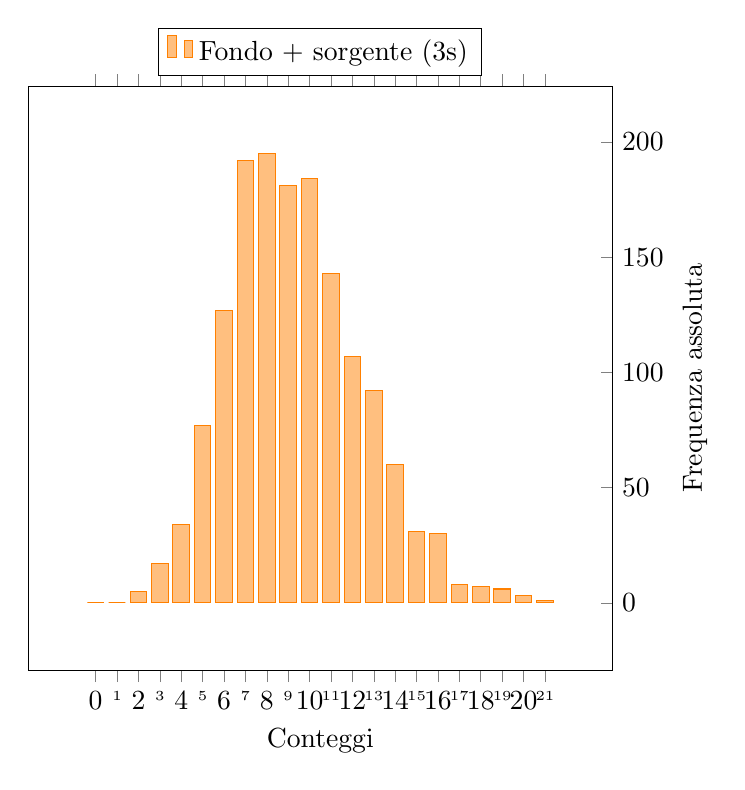
\begin{tikzpicture}
\begin{axis}[
	width=9cm, 
	height=9cm,
	ylabel=Frequenza assoluta,
	xlabel=Conteggi,
	enlargelimits=0.15,
	legend style={at={(0.5,1.1)},	anchor=north,legend columns=-1},
	ybar=0pt,  % configures `bar shift'
	bar width=6pt,
	xtick={0,1,2,3,4,5,6,7,8,9,10,11,12,13,14,15,16,17,18,19,20,21},
	xticklabels={0,\tiny{1},2,\tiny{3},4,\tiny{5},6,\tiny{7},8,\tiny{9},10,\tiny{11},12,\tiny{13},14,\tiny{15},16,\tiny{17},18,\tiny{19},20,\tiny{21}},
	xticklabel style={rotate=0, align=center},
	ytick pos=right]
	\addplot+[opacity=0.5,fill=orange,draw opacity=1,draw=orange] 
	coordinates {
		(0,0)
		(1,0)
		(2,5)
		(3,17)
		(4,34)
		(5,77)
		(6,127)
		(7,192)
		(8,195)
		(9,181)
		(10,184)
		(11,143)
		(12,107)
		(13,92)
		(14,60)
		(15,31)
		(16,30)
		(17,8)
		(18,7)
		(19,6)	
		(20,3)
		(21,1)};
	\legend{Fondo + sorgente (3s)}
\end{axis}
\end{tikzpicture}
\end{center}
\end{minipage}

\vspace{1cm}
A questo punto posso calolare il rate della sola sorgente per i due tempi porta prendendo il rate del fondo + sorgente e sottraendo ad esso il rate del fondo. 

Chiamati $FS$ fondo + sorgente e $F$ il fondo, l'incertezza associata alla sola sorgente si trova calcolando
\[
	\sqrt{\sigma_{FS}^2 + \sigma_{F}^2}
\]
si avrà il risultato desiderato calcolando
\[
	\text{Rate}_{FS} - \text{Rate}_F \pm \sqrt{\sigma_{FS}^2 + \sigma_{F}^2}
\]
Si trovano quindi due rate differenti ma apparentemente confrontabili. Mi aspetto infatti che i due rate siano uguali e che eventuali differenze tra i due siano dovute unicamente al caso. Ne verificherò la compatibilità nel punto 6 tramite un test Z.

\[
	(1s) \qquad \text{Rate}_{S1} = 2.78 \pm 0.05 \qquad \text{count}/s
\]

\[
	(3s) \qquad \text{Rate}_{S3} =  2.81 \pm 0.03  \qquad \text{count}/s
\]

\subsubsection*{La varianza e la media sono confrontabili entro 1,2,3,... volte la somma delle loro incertezze?}
Nel punto 5 tramite il test del chi quadro appurerò che la distribuzione teorica di Poisson si adatta ad entrambe le distribuzioni sperimentali dei conteggi del fondo più la sorgente radioattiva e, poiché nella poissoniana media e varianza sono uguali, posso cominciare a verificare l'adattamento delle distribuzioni sperimentali confrontando questi due valori (seppur non si tratti di un vero e proprio test statistico è utile per una verifica iniziale). 

Attingendo dai dati riportati in \textit{Tabella 3} e \textit{Tabella 4} si evince che per entrambi i tempi porta la differenza tra media e varianza è, in valore assoluto, minore della somma delle rispettive incertezze. 
\[
	\text{con} \quad \sigma_{\text{var}} = \frac{2\sigma_x^2}{\sqrt{2(N-1)}}
\]
\[
	(1s) \qquad |\bar{x} - \sigma_x^2| = 	|3.061 - 3.192| = \mathbf{0.131  < 0.163} = |0.046 + 0.117| =|\sigma_{\bar{x}} + \sigma_{\text{var}}| 
\]
\[
	(3s) \qquad |\bar{x} - \sigma_x^2| = 	|9.343 - 9.562| = \mathbf{0.219  < 0.429} = |0.080 + 0.349| =|\sigma_{\bar{x}} + \sigma_{\text{var}}| 
\]

% CHI QUADRO
\newpage
\section{Test \texorpdfstring{\(\chi^2\)}{chi}}
Tramite il test del \(\chi^2\) verifico se le distribuzioni teoriche di Poisson e di Gauss si adattano a quelle sperimentali calcolate con tempo porta di 1 secondo. \\

\noindent
Scelgo un livello di significatività $\alpha = 5\%$ e calcolo i rispettivi $\chi^2$ critici e i gradi di libertà.




\subsection{Adattamento a Poissoniana (1s)}
\paragraph{Ipotesi nulla} La distribuzione teorica di Poisson si adatta alla distribuzione sperimentale dei conteggi radioattivi misurati con tempo porta di 1s. 

\vspace{0.2cm}
\begin{center}
\begin{tabular}{lr}
	Numero classi & $10$ \\
	Livello di significatività $\alpha$		& $ \quad 5\%$  \\
	Valore di $\chi ^2$             	& $\quad 8.813$       \\
	Numero di gradi di libertà      	& $\quad (10-1-1) = 8$         \\   
	Valore di $\chi ^2$ critico     	& $\quad 15.507$
\end{tabular}
\captionof{table}{\textit{$\chi^2$ Poissoniana}}
\end{center}

\paragraph{Coclusione del test} Poiché $\chi^2 < \chi^2_{\text{critico}}$, la discrepanza tra le frequenze attese e quelle osservate risulta essere accettabile nei livelli di significatività scelti. Posso dire che la distribuzione teorica di Poisson si adatta bene alla distribuzione sperimentale e quindi \textbf{accetto} l'ipotesi nulla.

\begin{center}
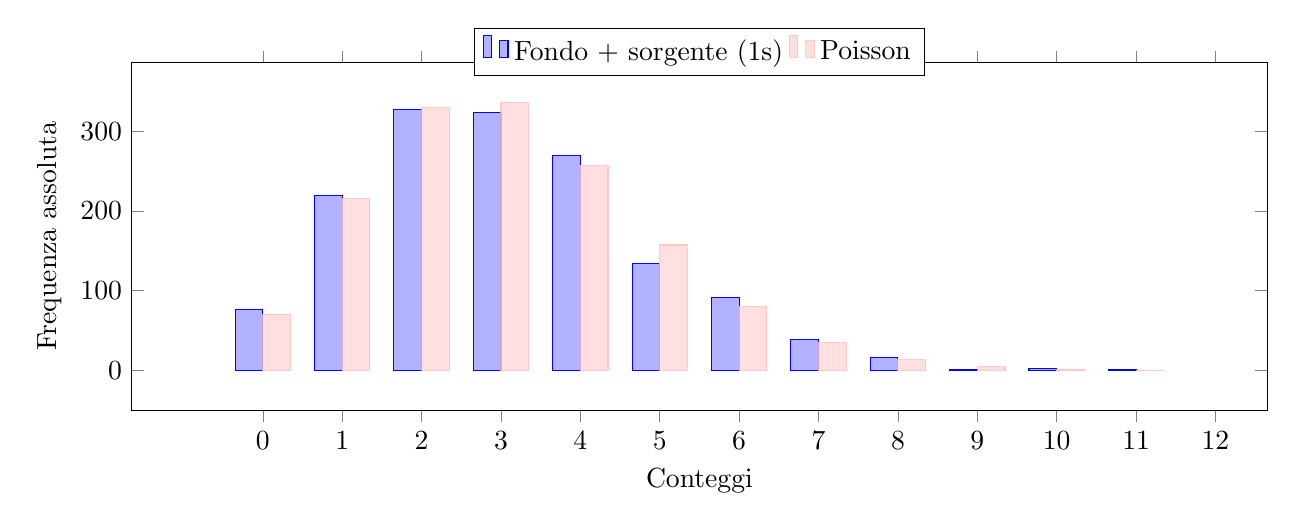
\begin{tikzpicture}
\begin{axis}[
	width=16cm, 
	height=6cm,
	ylabel=Frequenza assoluta,
	xlabel=Conteggi,
	enlargelimits=0.15,
	legend style={at={(0.5,1.1)},	anchor=north,legend columns=-1},
	ybar=0pt,  % configures `bar shift'
	bar width=10pt,
	xtick={0,1,2,3,4,5,6,7,8,9,10,11,12,13,14},
	xticklabels={0,1,2,3,4,5,6,7,8,9,10,11,12,13,14},
	xticklabel style={rotate=0, align=center}]
	\addplot+[opacity=1] 
	coordinates {
		(0,76)
		(1,219)
		(2,327)
		(3,323)
		(4,269)
		(5,134)
		(6,92)
		(7,39)
		(8,16)
		(9,1)
		(10,3)
		(11,1)};
	\addplot+[opacity=0.5,fill=pink,draw opacity=0.8,draw=pink]
	coordinates{
		(0,70.285)
		(1,215.118)
		(2,329.202)
		(3,335.859)
		(4,256.988)
		(5,157.311)
		(6,80.246)
		(7,35.087)
		(8,13.424)
		(9,4.565)
		(10,1.397)
		(11,0.389)};
	\legend{Fondo + sorgente (1s),Poisson};
\end{axis}
\end{tikzpicture}
\end{center}



\subsection{Adattamento a Gaussiana (1s)}
\paragraph{Ipotesi nulla} La distribuzione teorica di Gauss si adatta alla distribuzione sperimentale dei conteggi radioattivi misurati con tempo porta di 1s.

\vspace{0.2cm}
\begin{center}
\begin{tabular}{lr}
	Numero classi & $11$ \\
	Livello di significatività $\alpha$		& $ \quad 5\%$  \\
	Valore di $\chi ^2$             	& $\quad 96.060$       \\
	Numero di gradi di libertà      	& $\quad (11-2-1) = 8$         \\   
	Valore di $\chi ^2$ critico     	& $\quad 15.507$
\end{tabular}
\captionof{table}{\textit{$\chi^2$ Gaussiana}}
\end{center}

\paragraph{Coclusione del test} Poiché $\chi^2 > \chi^2_{\text{critico}}$ la discrepanza tra le frequenze attese e quelle osservate supera i valori accettabili nei livelli di significatività scelti. Posso dire che la distribuzione teorica di Gauss non si adatta alla distribuzione sperimentale e quindi \textbf{rigetto} l'ipotesi nulla.

\begin{center}
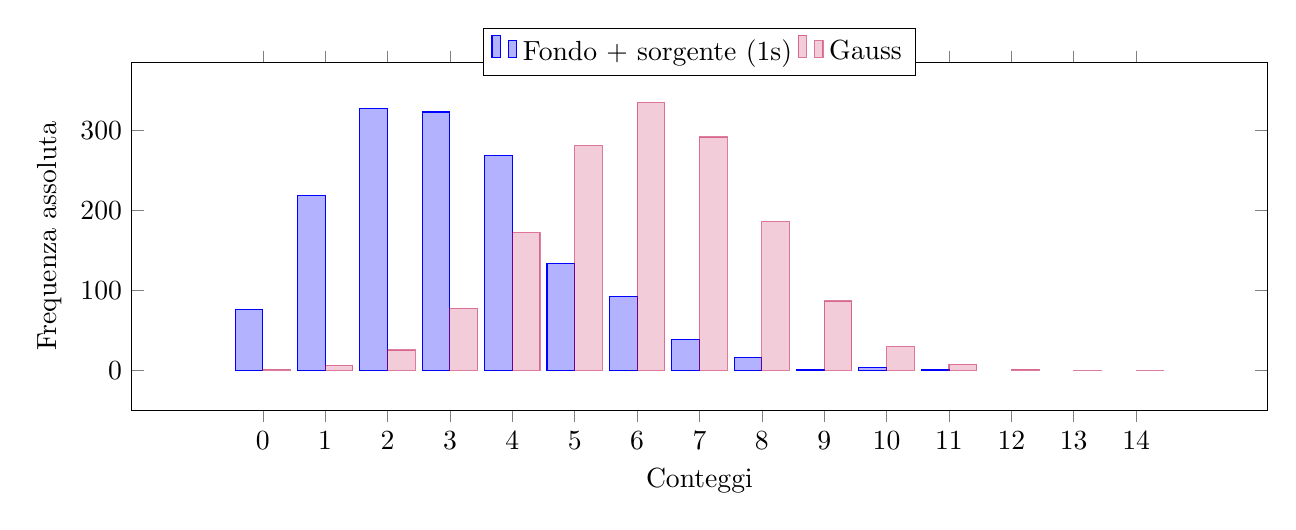
\begin{tikzpicture}
\begin{axis}[
	width=16cm, 
	height=6cm,
	ylabel=Frequenza assoluta,
	xlabel=Conteggi,
	enlargelimits=0.15,
	legend style={at={(0.5,1.1)},	anchor=north,legend columns=-1},
	ybar=0pt,  % configures `bar shift'
	bar width=10pt,
	xtick={0,1,2,3,4,5,6,7,8,9,10,11,12,13,14},
	xticklabels={0,1,2,3,4,5,6,7,8,9,10,11,12,13,14},
	xticklabel style={rotate=0, align=center}]
	\addplot+[opacity=1] 
	coordinates {
		(0,76)
		(1,219)
		(2,327)
		(3,323)
		(4,269)
		(5,134)
		(6,92)
		(7,39)
		(8,16)
		(9,1)
		(10,3)
		(11,1)};
	\addplot+[opacity=0.2,fill=purple,draw opacity=0.5,draw=purple]
	coordinates{
		(0,1.063)
		(1,6.067)
		(2,25.315)
		(3,77.225)
		(4,172.229)
		(5,280.813)
		(6,334.726)
		(7,291.691)
		(8,185.831)
		(9,86.552)
		(10,29.471)
		(11,7.336)
		(12,1.335)
		(13,0.178)
		(14,0.017)};
	\legend{Fondo + sorgente (1s),Gauss};
\end{axis}
\end{tikzpicture}
\end{center}



\subsection{Adattamento a Poissoniana (3s)}
\paragraph{Ipotesi nulla} La distribuzione teorica di Poisson si adatta alla distribuzione sperimentale dei conteggi radioattivi misurati con tempo porta di 3s.

\vspace{0.2cm}
\begin{center}
\begin{tabular}{lr}
	Numero classi & $17$ \\
	Livello di significatività $\alpha$		& $ \quad 5\%$  \\
	Valore di $\chi ^2$             	& $\quad 19.371$       \\
	Numero di gradi di libertà      	& $\quad (17-1-1) = 15$         \\   
	Valore di $\chi ^2$ critico     	& $\quad 24.996$
\end{tabular}
\captionof{table}{\textit{$\chi^2$ Poissoniana}}
\end{center}

\paragraph{Coclusione del test} Poiché $\chi^2 < \chi^2_{\text{critico}}$, la discrepanza tra le frequenze attese e quelle osservate risulta essere accettabile nei livelli di significatività scelti. Posso dire che la distribuzione teorica di Poisson si adatta bene alla distribuzione sperimentale e quindi \textbf{accetto} l'ipotesi nulla.

\begin{center}
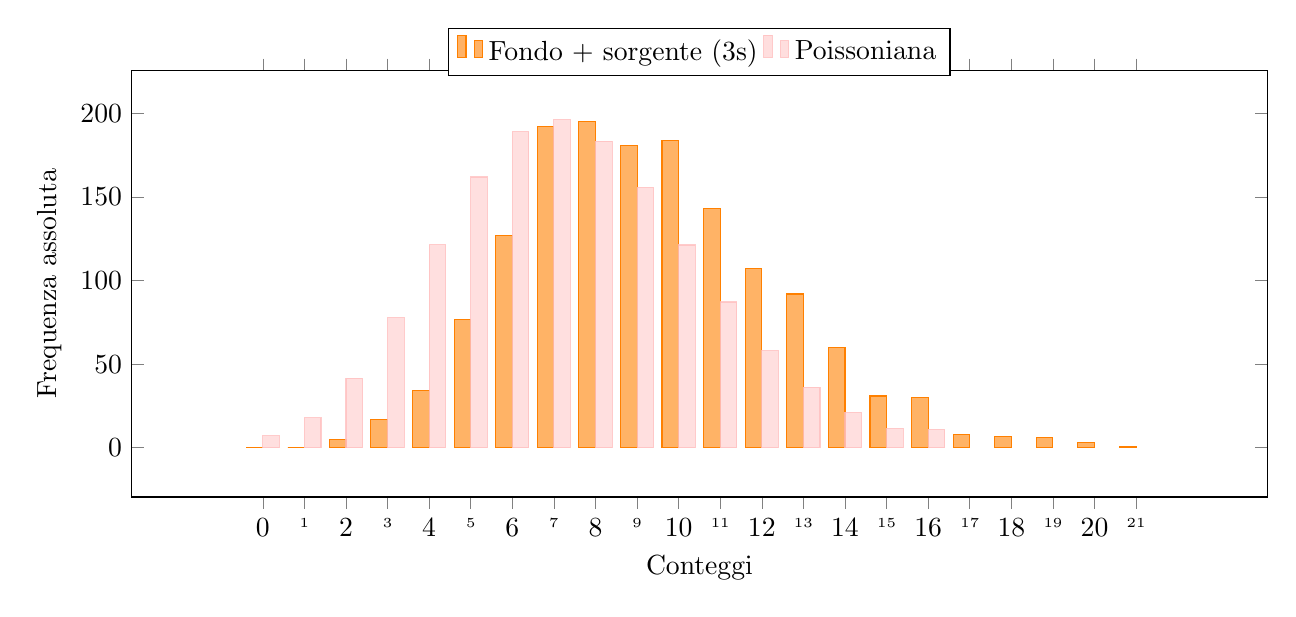
\begin{tikzpicture}
\begin{axis}[
	width=16cm, 
	height=7cm,
	ylabel=Frequenza assoluta,
	xlabel=Conteggi,
	enlargelimits=0.15,
	legend style={at={(0.5,1.1)},	anchor=north,legend columns=-1},
	ybar=0pt,  % configures `bar shift'
	bar width=6pt,
	xtick={0,1,2,3,4,5,6,7,8,9,10,11,12,13,14,15,16,17,18,19,20,21},
	xticklabels={0,\tiny{1},2,\tiny{3},4,\tiny{5},6,\tiny{7},8,\tiny{9},10,\tiny{11},12,\tiny{13},14,\tiny{15},16,\tiny{17},18,\tiny{19},20,\tiny{21}},
	xticklabel style={rotate=0, align=center}]
	\addplot+[opacity=0.6,fill=orange,draw opacity=1,draw=orange] 
	coordinates {
		(0,0)
		(1,0)
		(2,5)
		(3,17)
		(4,34)
		(5,77)
		(6,127)
		(7,192)
		(8,195)
		(9,181)
		(10,184)
		(11,143)
		(12,107)
		(13,92)
		(14,60)
		(15,31)
		(16,30)
		(17,8)
		(18,7)
		(19,6)
		(20,3)
		(21,1)};
	\addplot+[opacity=0.5,fill=pink,draw opacity=0.8,draw=pink]
	coordinates{
		(0, 7.092)
		(1, 17.857)
		(2, 41.708)
		(3, 77.936)
		(4, 121.359)
		(5, 161.978)
		(6, 189.169)
		(7, 196.378)
		(8, 183.475)
		(9, 155.836)
		(10, 121.331)
		(11, 87.199)
		(12, 58.193)
		(13, 36.246)
		(14, 21.165)
		(15, 11.632)
		(16, 11.011)};
	\legend{Fondo + sorgente (3s),Poissoniana};
\end{axis}
\end{tikzpicture}
\end{center}

\subsection{Adattamento a Gaussiana (3s)}
\paragraph{Ipotesi nulla} La distribuzione teorica di Gauss si adatta alla distribuzione sperimentale dei conteggi radioattivi misurati con tempo porta di 3s.

\vspace{0.2cm}
\begin{center}
\begin{tabular}{lr}
	Numero classi & $18$ \\
	Livello di significatività $\alpha$		& $ \quad 5\%$  \\
	Valore di $\chi ^2$             	& $\quad 59.344$       \\
	Numero di gradi di libertà      	& $\quad (18-2-1) = 15$         \\   
	Valore di $\chi ^2$ critico     	& $\quad 24.966$
\end{tabular}
\captionof{table}{\textit{$\chi^2$ Gaussiana}}
\end{center}

\paragraph{Coclusione del test} Poiché $\chi^2 > \chi^2_{\text{critico}}$ la discrepanza tra le frequenze attese e quelle osservate supera i valori accettabili nei livelli di significatività scelti. Posso dire che la distribuzione teorica di Gauss non si adatta alla distribuzione sperimentale e quindi \textbf{rigetto} l'ipotesi nulla.



\begin{center}
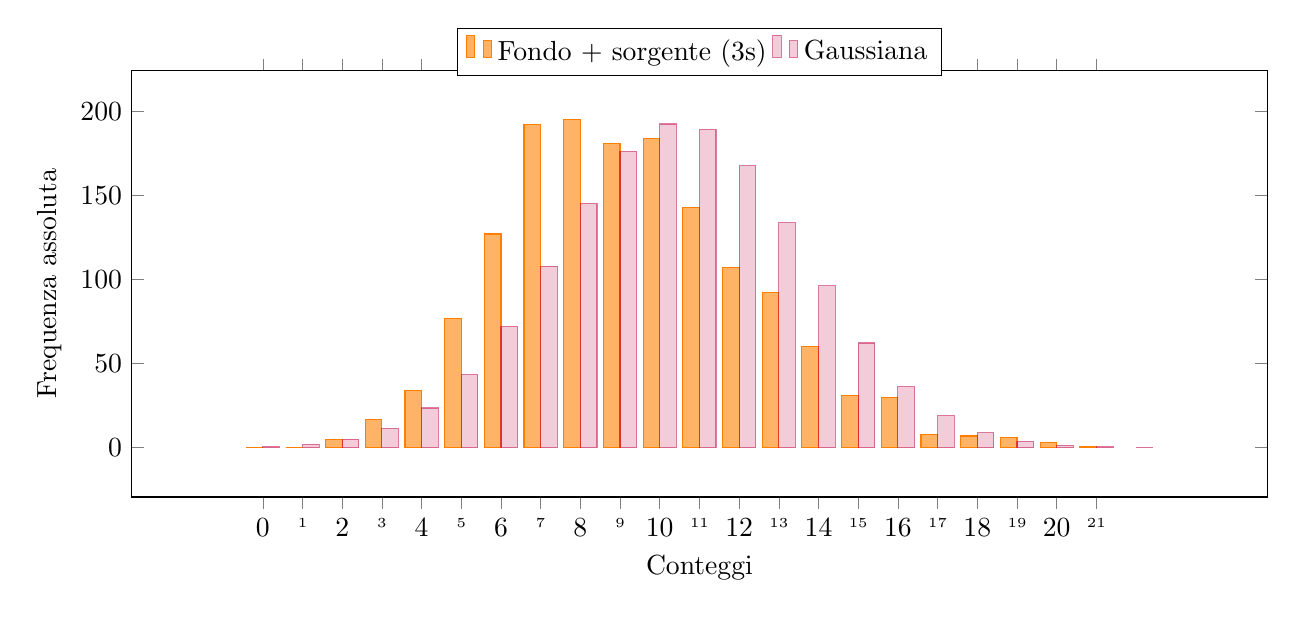
\begin{tikzpicture}
\begin{axis}[
	width=16cm, 
	height=7cm,
	ylabel=Frequenza assoluta,
	xlabel=Conteggi,
	enlargelimits=0.15,
	legend style={at={(0.5,1.1)},	anchor=north,legend columns=-1},
	ybar=0pt,  % configures `bar shift'
	bar width=6pt,
	xtick={0,1,2,3,4,5,6,7,8,9,10,11,12,13,14,15,16,17,18,19,20,21},
	xticklabels={0,\tiny{1},2,\tiny{3},4,\tiny{5},6,\tiny{7},8,\tiny{9},10,\tiny{11},12,\tiny{13},14,\tiny{15},16,\tiny{17},18,\tiny{19},20,\tiny{21}},
	xticklabel style={rotate=0, align=center}]
	\addplot+[opacity=0.6,fill=orange,draw opacity=1,draw=orange] 
	coordinates {
		(0,0)
		(1,0)
		(2,5)
		(3,17)
		(4,34)
		(5,77)
		(6,127)
		(7,192)
		(8,195)
		(9,181)
		(10,184)
		(11,143)
		(12,107)
		(13,92)
		(14,60)
		(15,31)
		(16,30)
		(17,8)
		(18,7)
		(19,6)
		(20,3)
		(21,1)};
	\addplot+[opacity=0.2,fill=purple,draw opacity=0.5,draw=purple]
	coordinates{
		(0, 0.720)
		(1, 2.015)
		(2, 5.082)
		(3, 11.541)
		(4, 23.607)
		(5, 43.494)
		(6, 72.177)
		(7, 107.880)
		(8, 145.233)
		(9, 176.105)
		(10, 192.335)
		(11, 189.202)
		(12, 167.638)
		(13, 133.783)
		(14, 96.164)
		(15, 62.259)
		(16, 36.305)
		(17, 19.069)
		(18, 9.021)
		(19, 3.844)
		(20, 1.475)
		(21, 0.510)
		(22, 0.159)};
	\legend{Fondo + sorgente (3s),Gaussiana};
\end{axis}
\end{tikzpicture}
\end{center}

\noindent
Durante l'analisi dati, nel calcolo del $\chi^2$ con modello gaussiano è risultato necessario attuare una normalizzazione dei dati da noi misurati con lo scopo di vere una somma delle frequenze assolute attese $\geq 1499.5$. Per fare ciò si sfrutta il fatto che la curva gaussiana abbia come dominio tutto $\mathbb{R}$, il che mi permette di aggiungere delle classi "vuote" con $x$ centrale negativo che normalizzano la somma delle frequenze assolute attese a circa 1500. Si aggiungono classi con conteggi negativi perché , come si può vedere dai grafici, ottenere un numero alto di conteggi è molto poco probabile e perciò le classsi con conteggi positivi successive a quelle già esistenti fornirebbero frequenze troppo basse e inutili al mio scopo.

\newpage
\section{Test di Gauss}
Ora voglio verificare l'accordo ottenuto tra i risultati dei rate per tempo porta di 1s e tempo porta di 3s. In linea teorica infatti mi aspetto che i due rate siano uguali e che eventuali discrepanze siano dovute unicamente al caso. Per il test calcolo la differenza in valore assoluto $\delta$ tra i due rate con la relativa incertezza e ne verifico la compatibilità con $\mu = 0$:


\[
	\delta = \left| \text{Rate}_{S1} - \text{Rate}_{S3} \right| \pm  \sqrt{\sigma_{S1}^2 + \sigma_{S3}^2}
\]

da cui ottengo

\[
	\delta = 0.03 \pm 0.06 \quad \text{count}/s	
\]

Calcolato $\delta$ scelgo un livello di significatività $\alpha = 5\%$ e procedo al calcolo dei valori di $z_{\text{osservato}}$ e $z_{\text{critico}}$.

\paragraph{Ipotesi nulla} $\delta$ assume un valore compatibile con quello di $\mu = 0$. 


\noindent
Calcolo il valore $\delta$ differenza tra il rate calcolato con tempo porta di 1s e il rate calcolato con tempo porta di 3s e l'incertezza associata:

\vspace{0.2cm}
\begin{center}
\begin{tabular}{lr}
	Livello di significatività $\alpha$	& $\quad 0.05$  \\
	Valore di $z_\text{oss}$             	& $\quad 0.50$  \\
	Valore di $z_{\text{critico}}$ 		& $\quad 1.96$  \\
	P-value 				& $\quad 0.62$  
\end{tabular}
\captionof{table}{\textit{$\chi^2$ Poissoniana}}
\end{center}

\paragraph{Conclusione del test} Come mostrato dai dati in \textit{Tabella 9} il valore del p-value è maggiore di $\alpha$, posso quindi accettare l'ipotesi nulla e affermare che $\delta$ è compatibile con $\mu = 0$ e di conseguenza i rate calcolati per tempi porta di 1 e 3 secondi sono confrontabili nei livelli di significatività scelti.  

\section{Conclusioni}
%E stato fatto un confronto tra liite gaussiana e poissoniana poiché ci aspettiamo una distribuzione poissoniana. Stimato il rate della sorgente a 3cm con tempi porta differenza. Due set di misure indipendenti è stato fatto un confronto per vedere di quanto il rate dei due set differisca se la differenza sia significativa se confrontata con errori casuali.





Ho misurato due set di dati rappresentanti il numero di conteggi registrati da un contatore geiger posto per tempi porta di 1 e 3 secondi raccogliendo 1500 misure degli eventi radioattivi dovuti alla radiazione naturale di fondo più la radiazione di una sorgente uranile.


Poi, poiché le mie aspettative riguardo la distribuzione dei conteggi erano quelle di avere distribuzioni ben descrivibili da una poissoniana, ho effettuato un test del $\chi^2$. Il test ha confermato che la distribuzione di Poisson si adatta a entrambe le distribuzioni sperimentali. 


Inoltre sapendo che al crescere del valor medio distribuzioni di Poisson possono tendere a una gaussiana ho ripetuto il test che ha però avuto esiti negativi portando alla conclusione che la distribuzione normale non si adatta a quella dei miei dati.\\


\noindent
Una volta stimato il rate della sorgente per entrambi i tempi porta ho confrontato i risulatati ottenuti per vedere quanto questi differiscano e se una eventuale discrepanza sia significativa o solo riconducibile a fluttuazioni statistiche. Ho quindi ottenuto:

\[
	(1s) \qquad \text{Rate}_{S1} = 2.78 \pm 0.05 \qquad \text{count}/s
\]

\[
	(3s) \qquad \text{Rate}_{S3} =  2.81 \pm 0.03  \qquad \text{count}/s
\]

dai quali calcolo una differenza $\delta$

\[
	\delta = 0.03 \pm 0.06 \quad \text{count}/s	
\]

A seguito di un test di Gauss questa risulta compatibile con $\mu = 0$ e perciò non significativa rispetto ai soli errori casuali.

\end{document}
